\scanpage{3}
\diagram{\begin{tikzcd}[column sep=small]
\unsure{k'}\arrow[ddr,no head,bend right=18]\arrow[rr,no head,bend left=45] & |[draw,ellipse]|\unsure{X}\arrow[dd] & \unsure{X_K}\arrow[l,Rightarrow]\arrow[dd,no head]\arrow[dd,no head,bend left=18]\\
&&\\
&\unsure{k}&\unsure{K}\arrow[l,no head]
\end{tikzcd}}

\figure{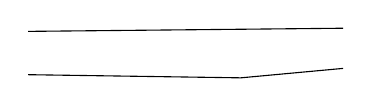
\begin{tikzpicture}
\draw (0,0)--(4,0.04);\draw (0,-.55)--(2.7,-.59)--(4,-.47);
\end{tikzpicture}}

\diagram{\begin{tikzcd}[column sep=small]
\unsure{Y}\arrow[r]\arrow[dr,no head]&X\arrow[d,no head]&&\unsure{Y'}\arrow[r]\arrow[dr,no head]&X'\arrow[d,no head]\\
&\unsure{k}\arrow[rrr,no head,"{\textcircled{\scriptsize\unsure{$\varphi$}}}"']&&{}\arrow[d]&\unsure{k'}\\
&&&{}&
\end{tikzcd}}

\diagram{\begin{tikzcd}
\unsure{Y}\arrow[d,"f"'] & \unsure{Y'}\arrow[l,"h"']\arrow[d,"f'"] & \unsure{V'}\\
X & X'\arrow[l,"g"',very thick]\arrow[d,no head,bend left=25] &\\
\unsure{g(U\prime)} & \unsure{U'\ne\varnothing}&
\end{tikzcd}}
\figure{\begin{tikzpicture}
\draw (0,0) .. controls (1,0.9) and (3,0.9) .. (4,0);
\draw (0,-.2) .. controls (-.3,-1) and (-.3,-2) .. (0,-2.5);
\end{tikzpicture}}

\diagram{\begin{tikzcd}
X'\arrow[r]\arrow[dr] &X\arrow[d,no head]\\
\unsure{\ne\varnothing}&\unsure{k}
\end{tikzcd}}

\diagram{\begin{tikzcd}
X\arrow[d,no head]&\\
\unsure{k}\arrow[r,no head]&Y
\end{tikzcd}}

\[
\unsure{A}\ -
\qquad
\begin{array}{c}
M\unsure{\subset|c}L\\
\times\,\unsure{M'U}
\end{array}
\]
\mspage{2}
